\chapter{Artigo: Receiver function imaging of mantle transition zone discontinuities beneath Parnaíba Basin}

Essa seção corresponde a segunda etapa do projeto, a qual consiste em observar as descontinuidades mantélicas de 410 km e 660 km, limites inferior e superior da Zona de Transição, abaixo da bacia do Parnaíba com as funções do receptor. Os limites da Zona de Transição e sua espessura são dependentes da temperatura, logo quando estão associados a anomalias termais essas descontinuidades de 410 km e 660 km devem ser imageadas a uma profundidade diferente da convencionada pelos modelos de velocidade globais. Para isso, apresentaremos empilhamentos e a migração em profundidade das funções do receptor para 9 estações na transecta NW-SE na parte central da bacia, como pode ser visto na Figura \ref{mapa_sta_mantle}.

\begin{figure}[!ht]
\begin{center}
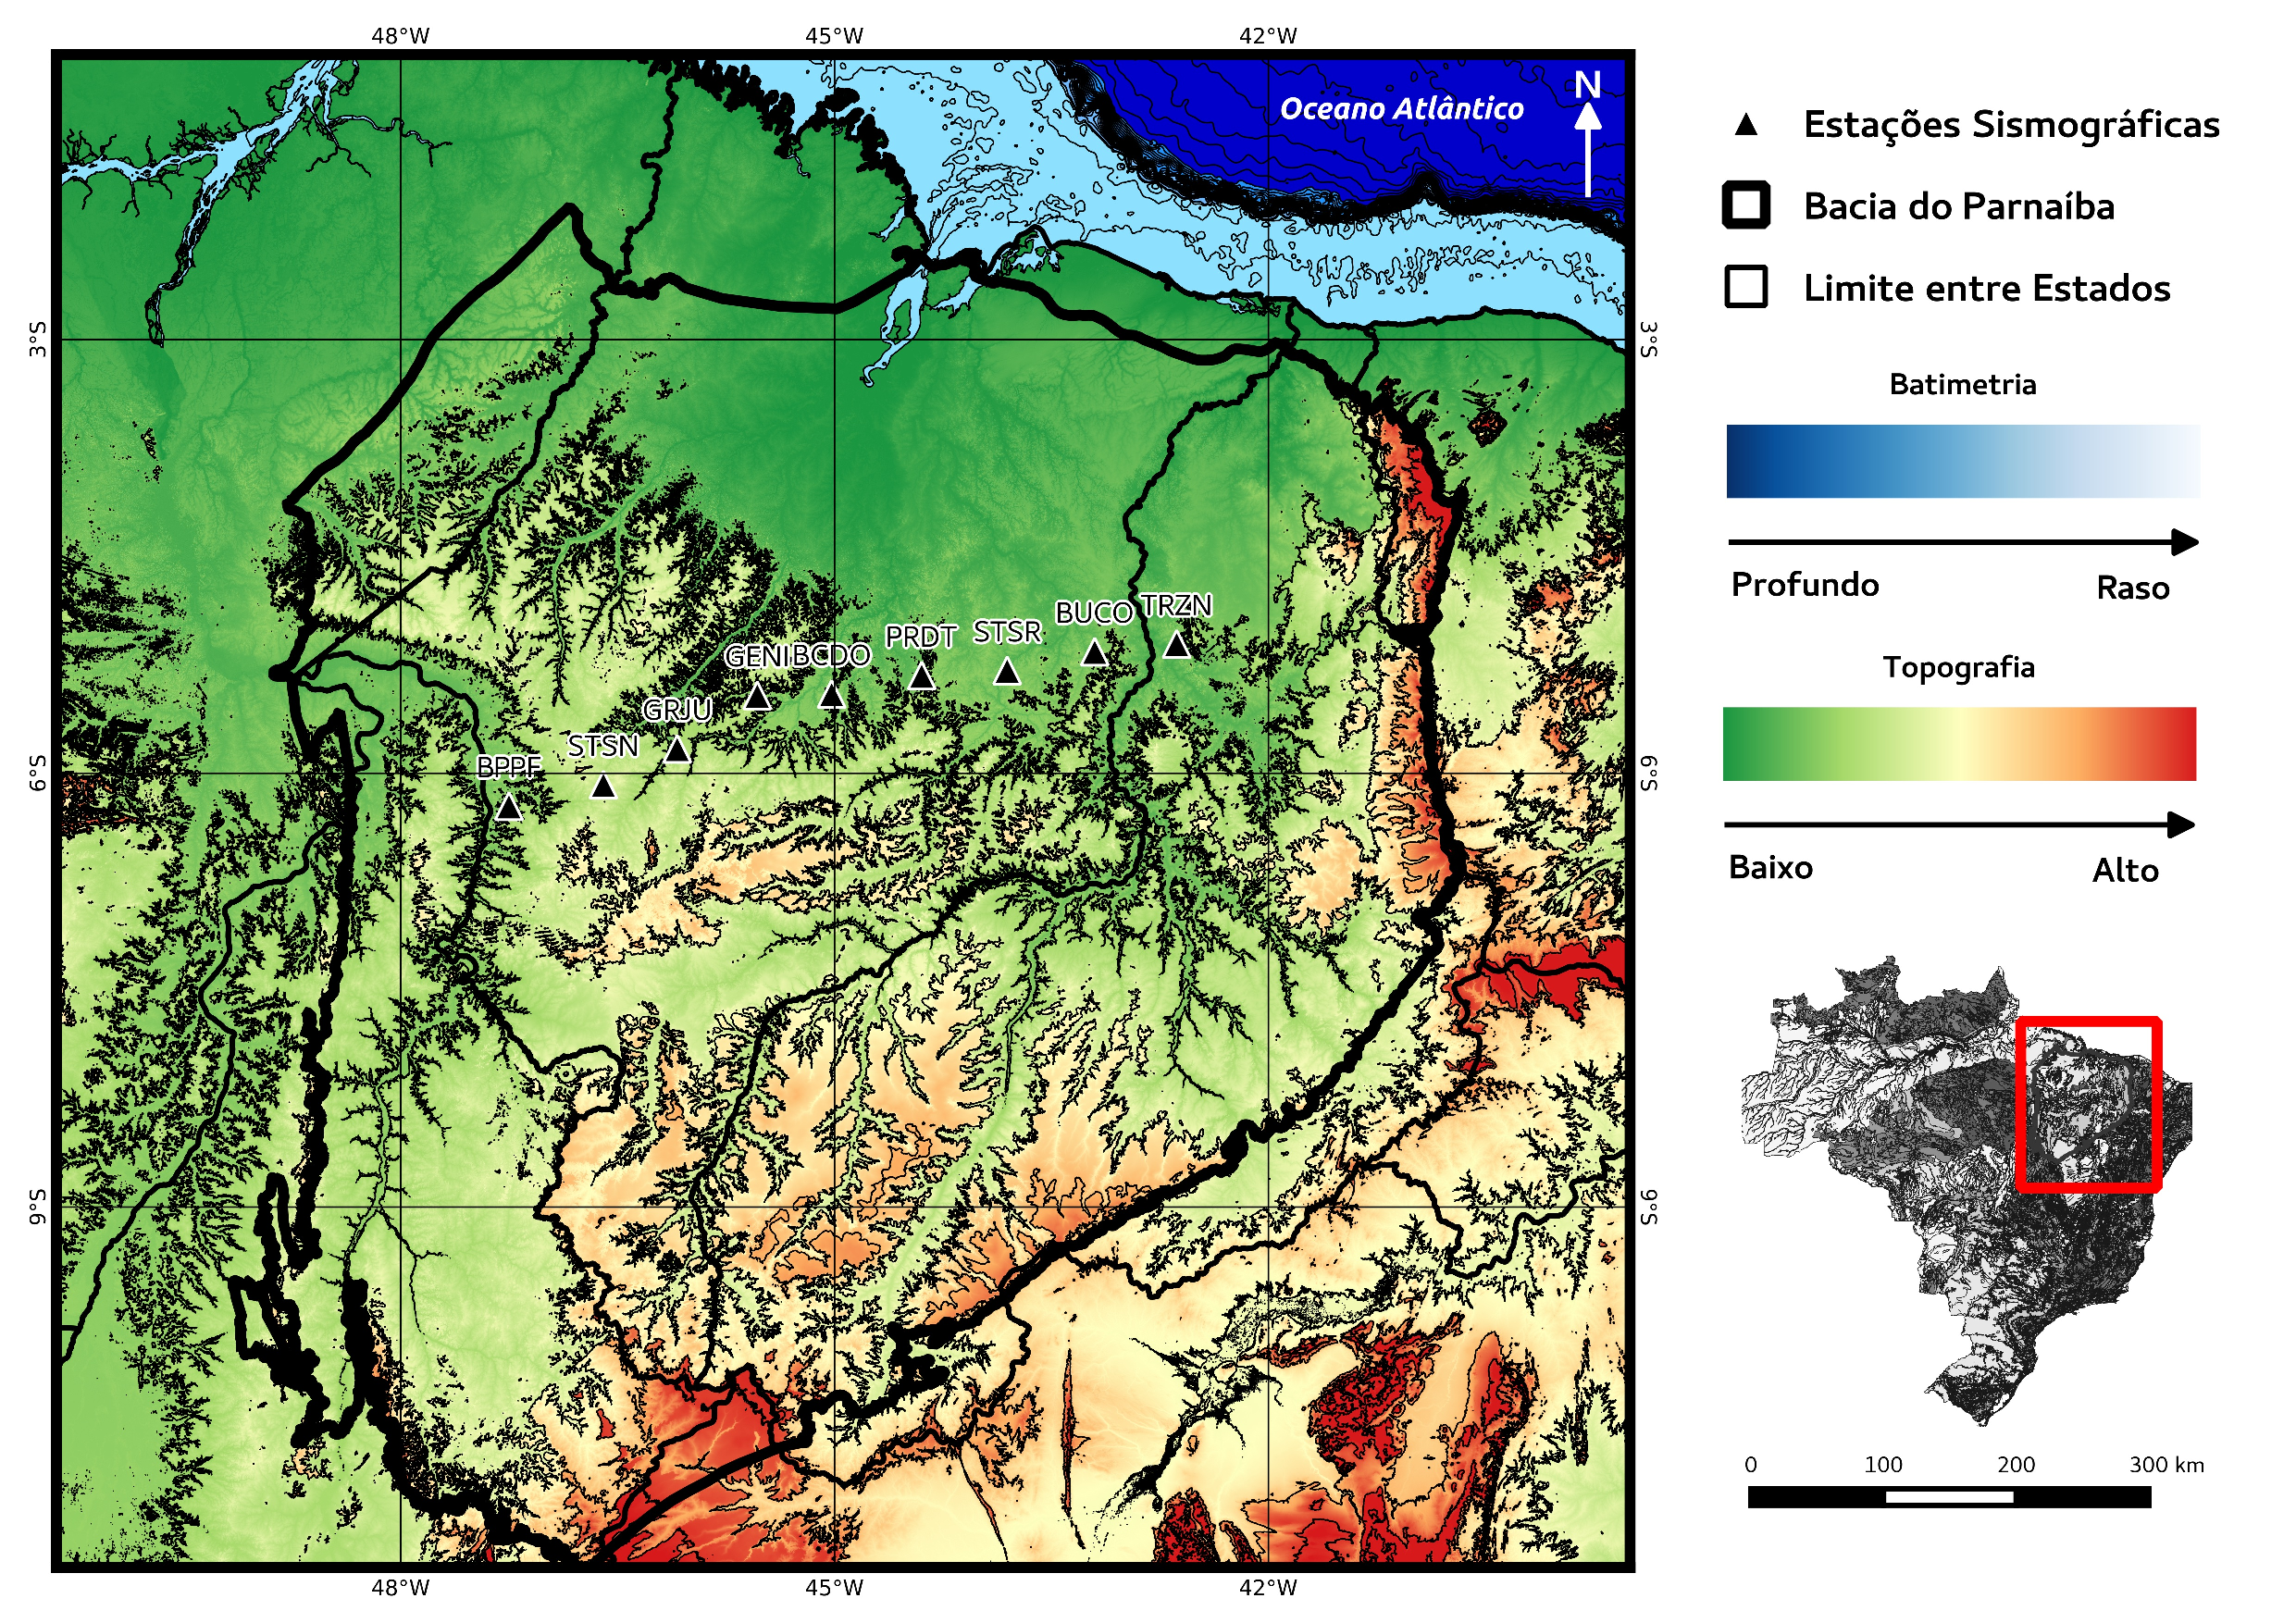
\includegraphics[width=1\textwidth]{Fig/mapa_topografico_estacoes.pdf}
\caption{Mapa com as estações da rede da BP na transecta NE-SW na Bacia do Parnaíba.}
\label{mapa_sta_mantle}
\end{center}
\end{figure}